\chapter{Background}
\label{ch:background}



\section{MathLang for Mathematics}
\label{sec:mathlangbackground}

\begin{enumerate}
\item \textit{MathLang is} \textbf{a framework.} It is meant to be used for communication as a concrete support for human mind formulation. MathLang is a well structured framework aimed to synthesize the common mathematical language.

\item \textit{MathLang is} \textbf{for mathematics}. It is meant to be open to any branch of mathematics and to any topic that uses mathematics as a base language. MathLang mimics mathematics in its incremental construction of a body of knowledge.

\item \textit{MathLang is} \textbf{for computerisation.} MathLang is meant to be a medium for a human-system, human-human via a digital support, and system-system communication. MathLang is a computer-based framework and therefore offers automation facilities.

Taken from Maarek's thesis \cite{manuelphd}.

MathLang's original Goals, when the project started in 2000 was to allow a gradual computerisation and formalisation of mathematical texts.

\end{enumerate}

MathLang is not a system for proof verification but a framework to computerise and translate information (such as mathematical text) into a form on which proof checkers can operate.

The MathLang framework provides extra features supporting more rigour to translation of the common mathematical language. One can define further levels of translations into more semantically and logically complete versions. This gradual computerisation method should be more accessible than direct formalisation, because a number of first levels do nor require any particular expertise in formalisation.

So far Mathlang has given alternative and complete paths which transform mathematical texts into new computerised and formalised versions. Dividing the formalisation of mathematical texts into a number of different stages was first proposed by N.G. de Bruijn to relate common mathematical language to his Mathematical Vernacular \cite{mv} and his proof checking system Automath.

\subsection{The Current MathLang Design \label{sec:currentmath}}
The MathLang Framework instructs the computerisation process to be broken up into a number of levels called \textbf{aspects}. Having an aspect prevents the misunderstanding of the process of computerisation of mathematical documents using the MathLang Framework. Each aspect can be worked out independently, simultaneously or sequentially without prior knowledge of another aspect. The current MathLang Framework contains three well-developed aspects, the \gls{cga}, the \gls{tsa} and the \gls{dra}, and has further aspects such as the Formal Proof Sketch.

\begin{figure}[H]
\begin{center}
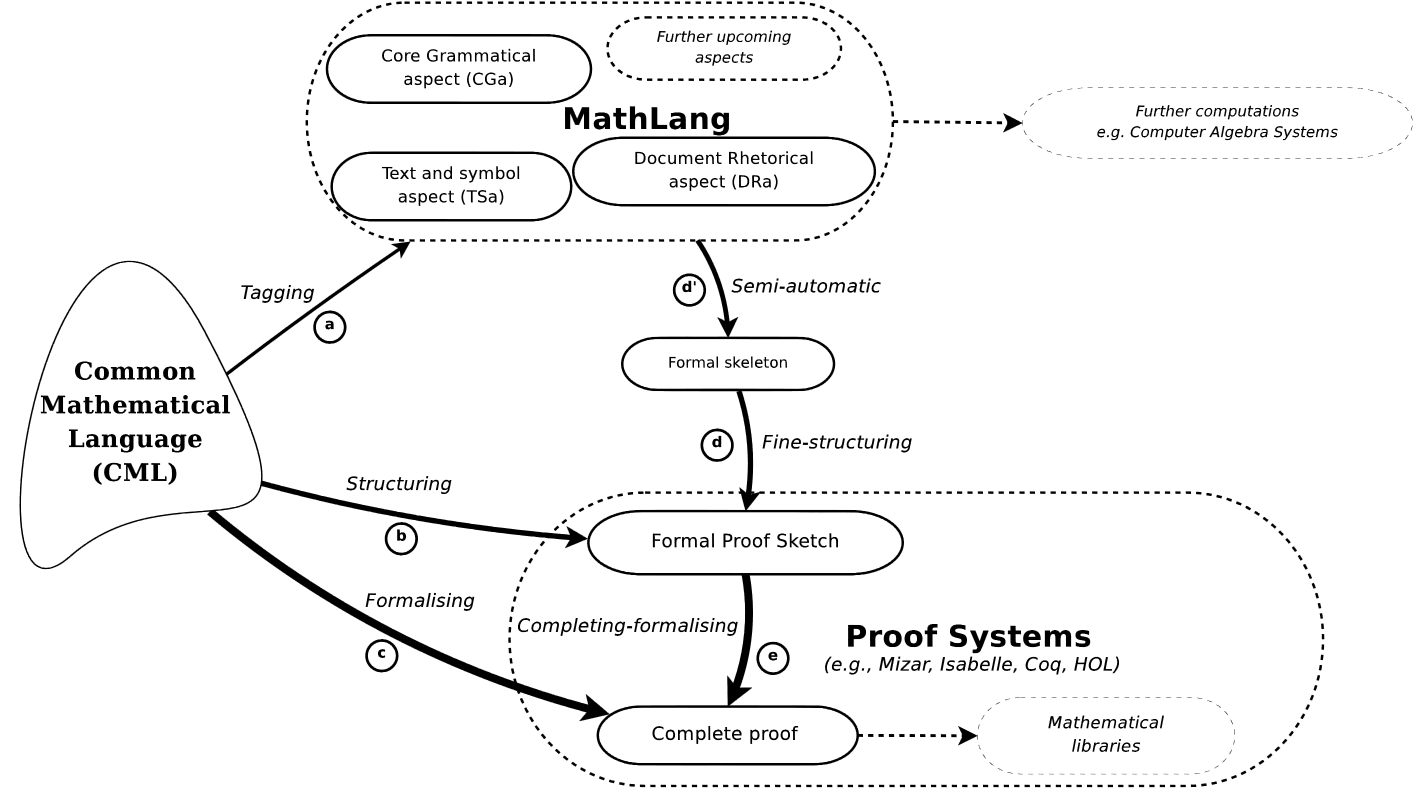
\includegraphics[scale=0.255]{Figures/Background/mathlang.png}
\end{center}
\caption{The MathLang approach to computerisation/formalisation \cite{mathintomizar}\label{fig:mathlang}}
\end{figure}

Figure \ref{fig:mathlang} shows the overall situation of work in the current MathLang Framework.
The labelled arrows show the computerisation paths from the common mathematical language to any proof system. The width of the arrow representing each path segment increases according to the expertise required to achieve the path segment. The level of expertise needed to computerise a CML text straight into a complete proof is very high, however the level of expertise is much smaller by using the MathLang framework to help form a formal skeleton and then into a complete proof. The dashed arrows illustrate further computerisation that one can envision.

\subsection{Core Grammatical aspect \label{subsec:cga}}
The current \gls{cga} in MathLang uses a finite set of grammatical \textit{categories} to identify the structure and common concepts used in mathematical texts. The aims of the \gls{cga} is to make explicit the grammatical role played by the elements of mathematical texts and to allow the validation of the grammatical and reasoning structure within the \gls{cga} encoding in a mathematical text. The \gls{cga} checks for grammatical correctness and finds errors like an identifier being used without and prior introduction or the wrong number of arguments being given to a function \cite{krzysztofphd}.

\subsection{Text and Symbol aspect \label{subsec:tsa}}
The \gls{tsa} builds the bridge between a mathematical text and its grammatical interpretation. The \gls{tsa} is a way of rewriting parts of the text so they have the same meaning. For example some mathematicians may prefer to write "a=b and b=c and c=d", others may prefer "a=b, b=c, c=d" and some others may prefer "a=b=c=d". As you can see all these methods of writing have the same meaning however some symbols are different. The \gls{tsa} annotates each expression in the text with a string of words or symbols which aim to act as the mathematical representation of which this expression is. This allows everything in the text to be uniform.

\subsection{Document Rhetorical aspect \label{subsec:dra}}

The Document Rhetorical aspects checks that the correctness of the reasoning in the mathematical document is correct and that there are no loops.The \gls{dra} mark-up system is simple and more concentrated on the narrative structure of the mathematical documents whereas other previous systems (such as DocBook \footnote{http://www.docbook.org}, Text Encoding Initiative \footnote{http://www.tei-c.org/index.xml}, OMDoc \footnote{http://www.omdoc.org}) were more concentrated on  the subtleties of the documents. It is used to describe and annotate chunks of texts according to their narrative role played within the document \cite{krzysztofphd}. Using the \gls{dra} annotation system we can capture the role that a chunk of text imposes on the rest of the document or on another chunk of text. This leads to generating dependency graphs which play an important role on mathematical knowledge representation. With these graphs, the reader can easily find their own way while reading the original text without the need to understand all of its subtleties. Processing \gls{dra} annotations can flag problems such as cicular reasoning and poorly-supported theorems.

\subsection{Full formalisation paths into Theorem Provers}

The MathLang project starts in 2000 when F.Kamareddine and J.B. Wells started the project within Heriot-Watt University as part of the ULTRA group \cite{researchprop}. It was an idea for a new mathematical language and framework to keep most of the advantages of Common Mathematical Language (CML) and avoid it's disadvantages. This framework would allow a gradual computerisation and formalisation of mathematical texts.

The framework was first set out in 2003 \cite{firstyear} and then saw an established path for conversion of a mathematical text written in CML into the isabelle proof assistant using rules and MathLang annotations \cite{secondyear}. A few short projects (by 4th year undergraduate dissertations or MSc students) have developed MathLang into the Framework it is today. A prototype of the Core Grammatical aspect and Text and Symbol aspect were defined in the PhD thesis of Manuel Maarek \cite{manuelphd} and then a gradual computerisation into the Mizar proof assistant using the three key aspects of MathLang were a great success and published \cite{mathintomizar}.

The design of the \gls{cga} is due to Kamareddine, Maarek and Wells \cite{oomathlang} and the implementation of the \gls{cga} is due to Maarek \cite{manuelphd}. The design of the \gls{tsa} is due to Kamareddine, Maarek, and Wells with contributions by Lamar to the souring rules \cite{restoringtsa}, \cite{manuelphd}, and \cite{lamarphd}. The implementation is primarily by Maarek \cite{manuelphd} with contributions from Lamar \cite{lamarphd}. The design and implementation of \gls{dra} were the subject of Retel's thesis \cite{krzysztofphd}. Further additions have since been carried out by Zengler \cite{cmtim}.

\subsection{Conclusion}
A lot of work has already been completed on the MathLang Framework. The three aspects, \gls{cga}, \gls{dra}, and \gls{tsa}, have been designed and redesigned so that a variety of mathematical texts and symbols could be used. Then the aspects have been implemented for ease of access. A translation from a mathematical text into the Mizar proof checker has been worked through and described in detail in a published paper \cite{mathintomizar} and a PhD thesis \cite{manuelphd}. A partial translation from a CML text into the Isabelle Syntax has also been carefully described in the 2009 paper \cite{mathintoisa} and also written in a PhD thesis \cite{lamarphd}. Some of the future work described was to allow MathLang to be used as a tool to computerise other pieces of information, such as another piece of academic text yet it does not need to be mathematical.

\section{Formal Methods in practice}
\label{sec:formnot}

Formal methods are mathematical approaches to software and system development which support the rigorous specification, design and verification of computer systems \cite{fmeurope}. Specifications are statements of how a proposed system should act and function. Formal methods use notations with defined mathematical meanings to describe specifications with prevision and no ambiguity. The properties of these specifications can then be works out with more confidence and can be described to the customers and other stakeholders. This then can uncover bugs in the stated requirements which they had not realised in a natural language specification. In this way a more complete requirements validation can take place earlier in the development life-cycle and thus save costs and time of the overall project. The rigor using formal methods eliminates design errors earlier and results in substantially redecued time \cite{benefitsofform}. 

Abrial presents two case studies in \cite{10.1145/1134285.1134406} describing the use of formal methods in industry. He concludes that one of the problems is that some managers are afraid that engineers will not be able to perform the interactive proofs. This thesis proposes to address this problem by inventing a method for a thereom proving novice to translate a formal specification into the theorem prover with little or no knowledge of the chosen theorem prover. The method proposed in this thesis provides an addition to testing and not a replacement. However the effort and costs should be reduced in the testing stages as the bugs would be found earlier in the specification and verification phase of the project. As well as giving the proposed system a highler level of rigor.

\subsection{The use of Formal Methods in Industry}

Despite these advantages some managers sometimes argue the cost of producing system using formal methods do not cover the costs. However the rigour using formal methods eliminates design errors earlier and results in substantially reduced time. Investing more effort in specifying, verifying and testing will benefit software projects by reducing maintenance costs, higher software reliability and more user-responsive software \cite{chantatub}.

Even in the 21st century we still experience a "software crisis" where software projects are being delivered far behind schedule, quality is poor and maintenance is expensive. Such software crisis allow for bad software to be released such as the computer system "Sabre" \cite{sabre}, which went off-line for almost a day leading to the cancellation of more then 700 flights.

Well engineered software is software which is suitable, efficient, reliable and maintainable with low costs and on schedule.

The cost of testing is around 50\% of the software cost. Maintenance cost is 2-4 times greater than pre-delivery cost. In large projects, failure to find and correct software errors can increase the cost of the software by 100 times, in small software projects it's usually about 2-4 times more.
More effort should be spent in requirements analysis and design to catch errors early in the project life-cycle \cite{andrewslides}. Computerising Z using the MathLang framework will do this as it is concentrating more on getting the requirement specifications correct and thus minimising errors later on in the project life cycle. For example, in the Sholis project \cite{sholis}, using a formal specification was most effective for fault finding, therefore if the specifications are correct, then the program implemented will in turn contain no grammatical errors if it follows the correct specification.

King, Hammond, Chapman and Pryor's paper \cite{sholis} was based on a project on the SHOLIS defence system. It highlighted the importance of having a Z specification on a system to check for errors. It was found that the Z proof was the most cost effective for fault finding. The Z specification found 75\% of the total faults for the system. Since Z specifications are important for finding faults in SIL4 systems (based on the sholis project), then checking the correctness of the Z specification is itself very important. Note that the specifications found 75\% of errors and not 100\%. As human error can still occur in formal specifications, using the ZMathLang approach may increase the percentage of errors found.

Hehner \cite{hehner99} also supports the use of specifications. He states it is the job of the specification to distinguish those things that are desirable in the program however when looking through a specification just with the human eye \cite{sholis} it is easy to make errors. Which is why checking the correctness of a specification through a theorem prover would help.

One reason industry is reluctant to use formal methods may be that they correctly perceive that the methods offered are too complicated for the benefits conferred. A way of simplifying the use of formal methods so that anyone in industry could understand would be a great benefit.

Hehner questions if all programs should have specifications. Which leads to the question of should simple programs also have specifications as well as high integrity systems. The benefits of planning and specifying a program far outweigh the time and cost of catching bugs and errors at a later stage \cite{planning} of complex programs. However it may be too time consuming for smaller program and it would be up to industry leaders themselves to decide.

Specifications, Programs, and Total Correctness \cite{hehner99} outlines that a programming language should not be the specification language. As not all industry experts are programming experts, the specification should be open for everyone in the team to understand the program not just the developers.

Hehner also states that total correctness is a mistake and partial correctness is enough. This may be because some software such as on aircraft's need to be running all the time when in the air and do not need to terminate. However with other programs it is important that they do terminate as a safety feature for example the Automatic track gauge changeover for trains \cite{automatictrain}. It is important that the program should terminate if anything should happen such as errors or a crash, therefore total correctness of only some programs is needed.

An Introduction to Proving the Correctness of Programs \cite{hantler} describes the specification of correct behaviour of a program by the use of input/output assertions. This would be very expensive in very large programs. So it may be good for smaller programs only. Assertion is a very basic approach.

However with this approach, checking for correctness can only be done by an expert in that particular programming language. They will have to understand where a procedure starts and where a procedure ends. By checking the correctness of specifications using the ZMathLang method it will allow for many program specifications to be checked by a wider audience and not just expert programmers.

The assumptions used in the example on page 336 \cite{hantler} resulted from an unresolved execution of the IF statement.

A paper reflecting on industry experience with proving properties in SPARK \ref{DBLP:conf/itp/ChapmanS14}, describes a programming language and verification system that will offer sound verification for programs. It states that SPARK and the use of proof tools remain a challange (published in 2014) as the `adoption hurdle' is percieved too high. Customers and regulators have taken a variety of stances on static analys and theorem provers. Where some places in industry have adopted the idea others remain sceptical. Hopefully this thesis will present an idea on how formal analysys could be simplified and broken up into smaller more understandable steps and thus would allow more users to take on the idea.

\section{Methods for checking for Software Correctness}

Traditionally, functional correctness has been obtained with pen and paper or an interactive proof assistant. Well-designed program verifiers are reducing the effort involved in doing full verifications.

Proof assistants soomestimes limit which program properties they reason about. By using the ZMathLang framework the specification would undergo different levels of rigor (and thus different types of checks) for example one might only want to check the grammatical correctness of the specification or one might want to fully formally prove the specification, different projects require different amounts of verification therefore the ZMathLang will allow this choice.

Dafny \cite{dafny} features modular verification, so that the separate verification of each part of the program implies the correctness of the whole program. This is similar to MathLang, Where Dafny checks different parts of the text and thus confirms confirms correctness of the full text, \gls{math} checks the correctness of the text through different levels of rigor.

Dafny was able to do a proof for the code of Schorr-Waited Algorithm, however the writer states that the loop invariants are complicated because they are concrete. A refinement approach such as Jean-Raymond Abrials approach \cite{abrial} may be preferred. This thesis presents a way of creating proofs for the program specifications in the essence of Z \cite{essenceofz} using the MathLang steps.  

The Java modelling language in Dafny lacks an automatic verifier. An automatic verifier for modelling languages in this case would be beneficial as pen and paper verification could have a bugs dues to human error.

Another attempt at checking for correctness was written by Rex L.Page in Engineering Software Correctness \cite{engineeringsoftwarecorrectness}. A general theme within this paper, is that design and quality are important in engineering education. When teaching students how to create programs, it is not enough just to teach them how to develop software but to develop good quality software. This paper describes experiments with the use of ACL2 (a subset of lisp) with embedded on mechanical logic to focus on design and correctness. By using ACL2 it emphasises the importance of software design and correctness. 

ALC2 is coded therefore users must know how to code software to formulate proofs. The intention of ZMathLang is to allow many people in the development team to be able to formulate proofs such as project managers, designers, engineers etc. To do this, The MathLang steps (see section \ref{sec:mathlangbackground}) should be simple to do and simple to understand.

PVS (Prototype Verification System) \cite{pvs} is an environment for constructing specifications and developing proofs which have been mechanically verified. PVS has it's own specification language, which engineers would need to learn as well as using the environment for proofs. Type checking is undecidable for the PVS type system. The PVS also provides a language for defining high-level inference strategies.

Another tool which analysis the Z notation is Hol-Z \cite{hol-z}. It is a proof environment for Z. Hol-Z is embedded in Isabelle/HOL therefore it provides a type checking, documentation facilities and refinement proofs with a trusted theorem prover. Tools for formal specifications can be a implement a specification environment into a programming language and an embedded design which implements it into a theorem prover. The Z specification is implemented in \LaTeX{} then typed checked using an external plug in Zeta then transformed into sml files to be added into the Hol-Z theorem prover environment. The user will need to have some good expertise in the theorem prover Isabelle/Hol in order to fully prove the specification.

Fuzz \cite{spiveyfuzz} is a typechecker for the original Z language. It includes style files for \LaTeX{} and checks for the logical correctness of Z specification. This is different to the \gls{zcga} type checker as the weak types in \gls{zcga} check for the grammatical correctness and not the full logical correctness of Z. Therefore the grammatical correctness of partially formal specification can aslo be checked. The \gls{zmath} framework presented in this thesis uses the `zed' \LaTeX{} style package to typeset the Z specifications in the documents.

These tools are just some of the many Z tools available. There are many other tools for Z which can be found on the Z Notation Wikia page \cite{zwikia}.

\section{Proof carrying-code}

Proof carrying code is a framework for the mechanical verification of safety properties in machine language programs. The provider of the Proof Carrying Code (PCC) must provide both the executable code and a machine-checkable proof. This is to ensure the safety of the executable code so that it doesn't access any other data it is supposed to. However the machine-checkable proof is often very large and going through these errors in the machine checkable proof can be very labour intensive. Appel \cite{fpcc} attempts to make this an easier method by using foundational proof carrying code where he avoids any commitment to a particular type system or a verification checker. MathLang is similar to this method as the ultimate aim of ZMathLang is for the specification is to go through a correctness check step by step and only at the very end pick a verification checker to translate to. However all the steps until the final three (see figure \ref{fig:steps}) do not require the user to commit to a particular theorem prover.

PPC has several characteristics that allow it to execute foreign code safely. A critical components of any PCC implementation is the safety policy which is specified right at the start before any implementation takes place. This policy uses safety rules that the consumer of the machine code desires for any untrusted code. Proof carrying code is a two stage verification process \cite{suappc}. Using a "proof producer" and a "code consumer" to do the work. The proof producer must produce two kinds of work, one is the machine code and the other is the proof to verify that the machine code is safely executable. The ultimate aim of \gls{zmath} is to translate the specification of the system into a theorem prover for a proof of the specification. Proof carrying code is slightly different as the proof comes with the code. Since a large system may have lots of different components which join to make one large system. The proof carrying code would need to be implemented in all of the components (or the most safety-dependent) components. Formal specifications usually display the entire system and it's individual components. Therefore the entire system as a whole would be checked. However for a higher level of rigor one can use the ZMathLang framework to chec for the correctness as a whole system and then using proof carrying code to check the code itself for correctness.

Manish Mahajan \cite{pccman} explains that any implementation of proof carrying code must contain at least 4 elements: (1) a formal specification language used to express the safety policy, (2) a formal semantics of the language used by the untrusted code, (3) a language used to express the proofs and (4) an algorithm for validating proofs. MathLang's Document Rhetorical aspect and Core Grammatical aspect could partially formalise the formal specification needed to express the safety policy, (1), then the rest of the steps would be easier to follow as they will need to be less specific.

Using fast, effective proof checkers can increase the speed of execution of the binary when the consumer has the added overhead of verification of the proof. Mahajan writes that the size of binary will be increased due to inclusion of the safety proof which is a major area for research, this safety proof can be done during the formal specification, when designing the prototype of the system and thus minimizing the size of the safety proof needed for the PCC.

\section{Z Syntax and Semantics}

The Z notation is based upon set theory and mathematical logic. It is a particular formal method to which was originally developed to specify the new Customer Information Control System (CICS) functionality \cite{cics}. The set theory includes standard set operators, set comprehensions, cartesian products and power sets. Z also has other aspects such as schemas which are used to group mathematical objects and their properties. The schema language can be used to describe the state of a system and the ways in which that state may change \cite{Woodcock:1996:UZS:235337}.

The semantics of Z specifications have already been studied. This has helped in the design of better specification languages by allowing critical comparison of specification techniques. As the basis semantics of Z have already been research, this gives us a head start in formulating the different aspects of \gls{math} for Z. The study in the semantics of Z provide a foundation for reasoning about specifications.

In \cite{formsem} it states that many of the proofs needed during the development process are `\textit{very shallow but contain a mass of detail}'. This detail would be difficult to understand by other stakeholders in the system being designed. This is where \gls{zmath} steps in, as it is a tool which produces documents in which anyone in the development team and clients should be able to understand.

The paper also states that \textit{consistency, completeness and refinement are essential to program development}. Therefore if the specification is consistent, complete and refined then the program will be as well (as long as the program sticks to the specification). Which makes it very important to have the specification checked as well as the program for errors. A formal semantics for the specification language is a necessary part of the specification of the software tools to support program development. Spivey also says that "theory  of signatures is decidable and therefore well suited to mechanical checking using a proof checker such as Mizar or Coq". However Mizar and Coq usually require a lot of expert level knowledge which leads to one of the aims of the thsis to break up the translation into smaller bitesize pieces to check for correctness of program specifications.

This thesis focuses on Ed Currie's, An Essence of Z \cite{essenceofz}. This would be a beneficial text to check for correctness as it only contains a subset of Z. Using the whole of Z may proof to be to difficult at the beginning as the syntax is very large and complicated, whilst starting with a small subset of Z and then expanding would be more efficient. The reason for this is because the framework developed in this thesis is for novices to get to grips with checking the correctness of Z and translating the specifications into a theorem prover. It does not promise to turn novices into theorem prover experts overnight but give them a guide with verifying the correctness of specifications. The research presented here is also not intended for theorem prover experts however users who are experts in theorem proving may also find some steps of the \gls{zmath} framework beneficial such as the \gls{zcga} or \gls{zdra}. The Essence of Z is also used as an academic text in undergraduate teaching and starts with very basics of logic to larger specifications which can be used a real software systems. It contains more then one specification and therefore gives a variety of syntax to use the MathLang framework on.

\section{Types and their desirable properties}

Type systems are good for many things \cite{pierce}, one of which includes that it allows early detection of some programming errors. Errors that are detected early can be fixed straight away rather then it lingering around to be discovered much later. Errors can often be pinpointed more accurately during type checking more often then in run-time, when their effects may not become visible until after some things go wrong, which in high integrity systems can have disastrous results. Type systems support the programming process by enforcing disciplined programming. Type system form the backbone of the module languages used to packaged and tie together all the different parts of large scale software systems. Types are also useful when reading programs. They form a useful documentation to the reader about the behaviour of the program, this form of documentation can not be outdated like comments since when the program specification changes so does the types involved.

Type-free lambda calculus \cite{bar93} allows for every expression to be applied to every other expression, eg I = $\lambda x.x$ may be applied to any argument $x$ to give the same result $x$. The expression may also be applied to itself. There are also typed versions of lambda calculus introduced by Curry \cite{cu34}. Types are usually objects of a syntactic nature and may be assigned to lambda terms. Using Types in this nature, this thesis describes a way in the \gls{zcga} (chapter \ref{ch:zcga}) assigns grammatical types to parts of a specification written in Z or partially written in Z. By doing so, the grammatical correctness of a system specification could be checked. The grammatical types are an adaptation from the grammatical categories taken from \cite{wtt}. One of the main benefits of the \gls{zcga} is it can check the grammatical correctness of partial formal specifications, that is specifications which are written in natural language and are on the way to becoming formal. Other Z type checkers such as Z/Eves \cite{Saaltink99thez/eves} and Fuzz \cite{spiveyfuzz} check the logical type correctness of a fully formalised Z specification.

\section{Generating properties to prove for Formal Specifications}
\todo[inline]{Explain different ways users can identify properties to prove for their Z specs}

\cite{DBLP:conf/icsea/WenMZ06}, \cite{DBLP:conf/sefm/FraserB07}, \cite{stepney1998tale}, \cite{Woodcock:1996:UZS:235337}, \cite{woodcock2004tutorial}

\section{Conclusion}
\todo[inline]{Write a conclusion for background chapter}